%*********************************************************************
% gdutthesis: 广东工业大学论文模板
% 2021/06/07 v0.1a
%
% 重要提示:
%   1. 请确保使用 UTF-8 编码保存
%   2. 请使用 XeLaTeX 或 LuaLaTeX 编译
%   3. 请仔细阅读用户文档
%   4. 修改、使用、发布本文档请务必遵循 LaTeX Project Public License
%   5. 不需要的注释可以尽情删除
%*********************************************************************
\documentclass[
  % type=doctor
  type=master
  % type=promaster
]{gdutthesis}

% 宏包在这里加载
\usepackage{siunitx,zhlipsum,lipsum}

\gdutsetup{
  style = {
    font            = {times},
    % font            = {times*},
    cjk-font        = {fandol},
    % cjk-font        = {founder},
    % cjk-font        = {mac},
    % cjk-font        = {sourcehan},
    % cjk-font        = {noto},
    % cjk-font        = {windows},
    % cjk-font        = {none},
    bib-backend     = {bibtex},
    % bib-backend     = {biblatex},
    bib-resource    = {gdutthesis-template.bib},
    bib-style       = {numerical},
    % bib-style       = {author-year},
    fullwidth-stop  = {mapping},
    % fullwidth-stop  = {catcode},
    % fullwidth-stop  = {false},
    hyperlink       = {color},
    % hyperlink       = {border},
    % hyperlink       = {none},
    hyperlink-color = {default},
    % hyperlink-color = {autumn},
    % hyperlink-color = {business},
    % hyperlink-color = {classic},
    % hyperlink-color = {elegant},
    % hyperlink-color = {fantasy},
    % hyperlink-color = {material},
    % hyperlink-color = {science},
    % hyperlink-color = {summer},
    % hyperlink-color = {graylevel},
    % hyperlink-color = {prl},
  },
  info = {
    title           = {模板射流电解加工微沟槽关键技术研究},
    title*          = {Investigation on masked jet electrochemical machining of micro grooves},
    date            = {2020/5/25},
    author          = {张三},
    author*         = {Zhang San},
    supervisor      = {李四\qquad 教授},
    supervisor*     = {Prof. Li Si},
    supervisor-two  = {王五\qquad 教授},
    supervisor-two* = {Prof. Wang Wu},
    department      = {自动化学院},
    department*     = {Automation},
    major           = {电子信息(控制工程方向)},
    student-id      = {2121001234},
    chairman        = {赵六\qquad 教授},
    degree          = {工学硕士},
    degree*         = {Master of Engineering Science},
    keywords        = {电解加工, 微沟槽, 模板, 射流},
    keywords*       = {electrochemical machining, micro grooves, mask, jet},
    secret-level    = {none},
  }
}


\begin{document}

\begin{abstract}
  \zhlipsum[1-4]
\end{abstract}

\begin{abstract*}
  \lipsum[1-4]
\end{abstract*}

\begin{notation}
  $E$ & 能量 \\
  $F$ & 推力
\end{notation}

\gduttableofcontents

\mainmatter

\gdutchapter{绪论}{Introduction}

\gdutsection{本课题研究背景及研究意义}{Background and significance of research}
随着科学技术的进步,产品逐渐向精密化和高性能化发展,具有毫米及微米尺度
微沟槽结构的金属零部件在国防军事、航空航天、新能源、新材料、生物医学、半导
体器件等领域的高技术产品中扮演的角色愈加重要。

\gdutsection{微沟槽电解加工国内外相关研究现状}{Analysis of the research status at home and abroad}
\gdutsubsection{成型电极电解加工}{Shaped cathode electrochemical machining}
采用与微沟槽结构形状对应的成型阴极,例如薄板阴极,片状阴极等,进行微沟
槽电解加工,其特点是方便一次成型微沟槽形状。南京航空航天大学吕焱明等进行了
大长宽比深窄槽电解加工阴极设计以及工艺试验研究\cite{feynman2011feynman},如\autoref{fig:example} 所示,具体参考\autoref{sub-fig-1} 和\autoref{sub-fig-2},再参考\autoref{eq:example},再再参考\autoref{tab:example}。
\begin{equation}\label{eq:example}
  E = mc^2
\end{equation}

\begin{figure}[htbp]
  \subfloat[贴有模板的金属喷嘴示意图]{\label{sub-fig-1}
    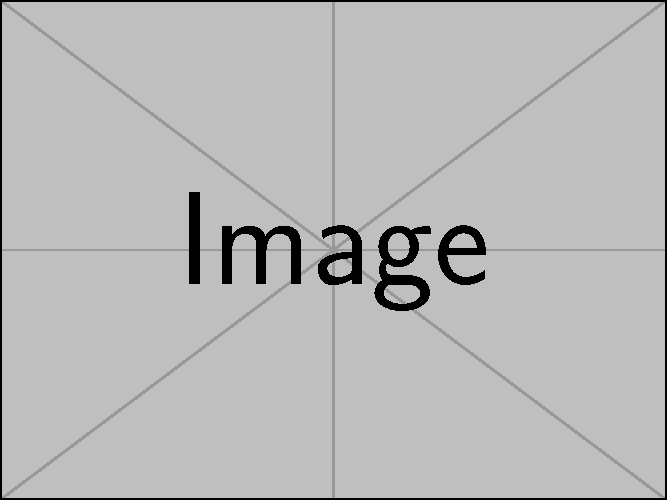
\includegraphics[width=0.4\textwidth]{example-image.pdf}
  }
  \qquad
  \subfloat[由点到线扫描加工原理图]{\label{sub-fig-2}
    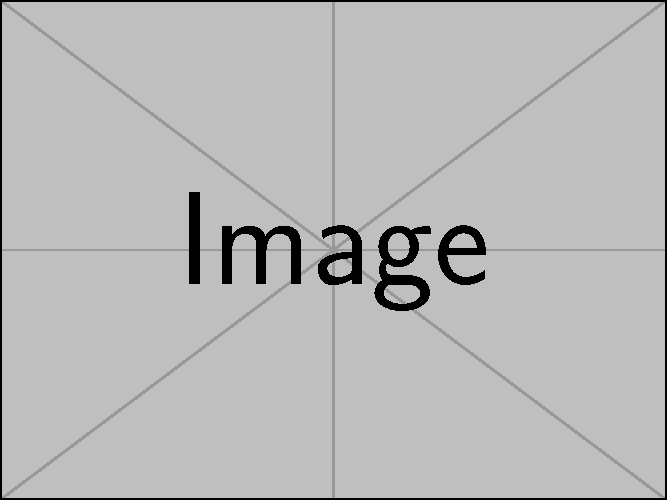
\includegraphics[width=0.4\textwidth]{example-image.pdf}
  }
  \bicaption{模板射流电解加工微沟槽原理图}{Principle of masked jet electrochemical machining of micro grooves}
  \label{fig:example}
\end{figure}

\begin{table}
  \bicaption{DMC5400A 运动控制卡主要技术指标}{DMC5400A main specifications}
  \label{tab:example}
  \begin{tabular}{cc}
    \toprule
    控制卡技术指标              & 具体参数                      \\
    \midrule
    控制电机的脉冲信号频率范围  & $\qty{1}{Hz}\sim\qty{2}{MHz}$ \\
    控制电机的脉冲信号频率精度  & \qty{0.0625}{Hz}              \\
    脉冲信号输出最大电流        & \qty{20}{mA}                  \\
    脉冲信号长度                & 28 位有符号                   \\
    直线插补精度                & $\pm \qty{0.8}{pulse}$        \\
    圆弧插补精度                & $\pm \qty{1.5}{pulse}$        \\
    支持的插补坐标系个数        & 2                             \\
    \bottomrule
  \end{tabular}
\end{table}


\subsubsection{微沟槽电解加工国内外相关研究现状}
测试 test。
\paragraph{测试 test。}
测试 test。
\subparagraph{测试 test。}
测试 test\cite{曾谨言2013量子力学}。

\gdutbackmatter
\gdutchapter{结论与展望}{Conclusion and prospect}
\gdutbacksection{研究结论}
\zhlipsum[1]

\gdutbacksection{未来研究展望}
\zhlipsum[1]

\printbibliography

\gdutchapter{攻读学位期间取得与学位论文相关的成果}{Publication and patents during study}

\gdutbacksection{发表和投稿与学位论文相关学术论文}

\begin{results}
  \item \textbf{张三}, 李四, 等. Jet electrochemical machining of micro dimples with conductive mask.
  Journal of Materials Processing Technology. 2018, 257:101-111. (SCI Impact Factor 3.647,
  WOS:000431161400010)
  \item 李四, \textbf{张三}, 王五, 等. Electrochemical direct-writing machining of micro- channel array.
  Journal of Materials Processing Technology. 2019, 265:138-149. (SCI Impact Factor 3.647,
  WOS:000451935100014)
\end{results}

\gdutbacksection{申请发明专利}

\begin{results}
  \item 李四, \textbf{张三}, 王五. 一种微流道电解加工装置. 发明专利申请号: 201810467763.5.
\end{results}

\gdutstatement

\gdutchapter{致谢}{Acknowlegements}
\zhlipsum[1]

\gdutappendix

\gdutchapter{附录标题}{The appendix title}
对需要收录于学位论文中且又不适合书写于正文中的附加数据、资料、详细
公式推导、计算机程序等有特色的内容,可做为附录排写。
\end{document}